\documentclass{article}
\usepackage[paperheight=14.6cm, paperwidth=5.5in, margin=0mm]{geometry}
\usepackage{tikz}
\usepackage{subfig}

\begin{document}

\begin{figure}
  \subfloat[Flow direction]{
    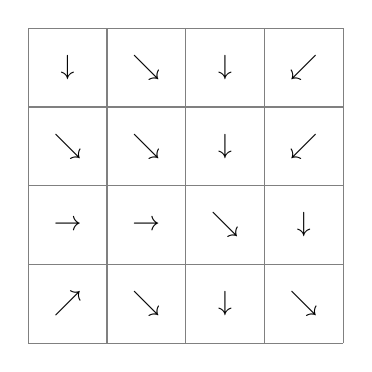
\begin{tikzpicture}
      \draw[step=1cm,color=gray] (-2,-2) grid (2,2);

      \node at (-1.5,+1.5) {$\downarrow$};
      \node at (-0.5,+1.5) {$\searrow$};
      \node at (+0.5,+1.5) {$\downarrow$};
      \node at (+1.5,+1.5) {$\swarrow$};

      \node at (-1.5,+0.5) {$\searrow$};
      \node at (-0.5,+0.5) {$\searrow$};
      \node at (+0.5,+0.5) {$\downarrow$};
      \node at (+1.5,+0.5) {$\swarrow$};

      \node at (-1.5,-0.5) {$\rightarrow$};
      \node at (-0.5,-0.5) {$\rightarrow$};
      \node at (+0.5,-0.5) {$\searrow$};
      \node at (+1.5,-0.5) {$\downarrow$};

      \node at (-1.5,-1.5) {$\nearrow$};
      \node at (-0.5,-1.5) {$\searrow$};
      \node at (+0.5,-1.5) {$\downarrow$};
      \node at (+1.5,-1.5) {$\searrow$};
    \end{tikzpicture}
  }
  \subfloat[Flow accumulation area]{
    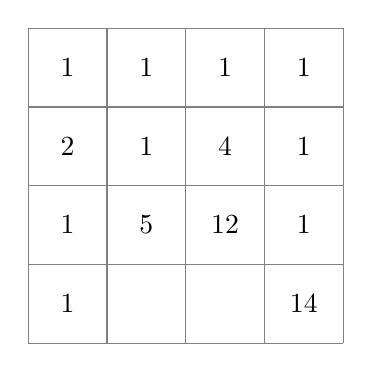
\begin{tikzpicture}
      \draw[step=1cm,color=gray] (-2,-2) grid (2,2);

      \node at (-1.5,+1.5) {$1$};
      \node at (-0.5,+1.5) {$1$};
      \node at (+0.5,+1.5) {$1$};
      \node at (+1.5,+1.5) {$1$};

      \node at (-1.5,+0.5) {$2$};
      \node at (-0.5,+0.5) {$1$};
      \node at (+0.5,+0.5) {$4$};
      \node at (+1.5,+0.5) {$1$};

      \node at (-1.5,-0.5) {$1$};
      \node at (-0.5,-0.5) {$5$};
      \node at (+0.5,-0.5) {$12$};
      \node at (+1.5,-0.5) {$1$};
      % ...
      \node at (-1.5,-1.5) {$1$};
      \node at (-0.5,-1.5) {};
      \node at (+0.5,-1.5) {};
      \node at (+1.5,-1.5) {$14$};
    \end{tikzpicture}
  }
  \subfloat[River centerline]{
    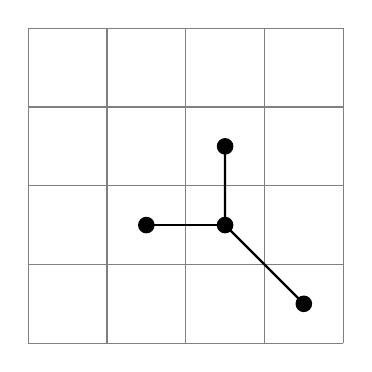
\begin{tikzpicture}
      \draw[step=1cm,color=gray] (-2,-2) grid (2,2);
      % Mark cells with flow accumulation ≥ 4 as red dots
      \fill[black] (0.5,0.5) circle (3pt);    % value 4
      \fill[black] (-0.5,-0.5) circle (3pt);  % value 5
      \fill[black] (0.5,-0.5) circle (3pt);   % value 12
      \fill[black] (1.5,-1.5) circle (3pt);   % value 14

      % Draw the main centerline along the highest accumulated path
      \draw[black,thick] (0.5,0.5) -- (0.5,-0.5) -- (1.5,-1.5);
      \draw[black,thick] (0.5,-0.5) -- (-0.5,-0.5);
    \end{tikzpicture}
  }

  \subfloat[Drainage density]{
    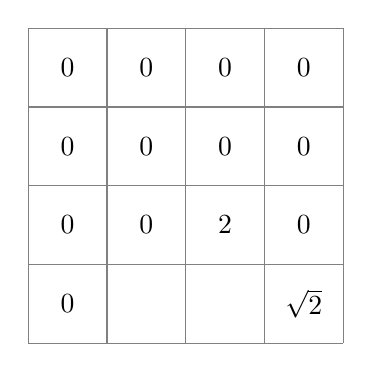
\begin{tikzpicture}
      \draw[step=1cm,color=gray] (-2,-2) grid (2,2);

      \node at (-1.5,+1.5) {$0$};
      \node at (-0.5,+1.5) {$0$};
      \node at (+0.5,+1.5) {$0$};
      \node at (+1.5,+1.5) {$0$};

      \node at (-1.5,+0.5) {$0$};
      \node at (-0.5,+0.5) {$0$};
      \node at (+0.5,+0.5) {$0$};
      \node at (+1.5,+0.5) {$0$};

      \node at (-1.5,-0.5) {$0$};
      \node at (-0.5,-0.5) {$0$};
      \node at (+0.5,-0.5) {$2$};
      \node at (+1.5,-0.5) {$0$};
      % ...
      \node at (-1.5,-1.5) {$0$};
      \node at (-0.5,-1.5) {};
      \node at (+0.5,-1.5) {};
      \node at (+1.5,-1.5) {$\sqrt{2}$};
    \end{tikzpicture}
  }
  \subfloat[Total upstream river length]{
    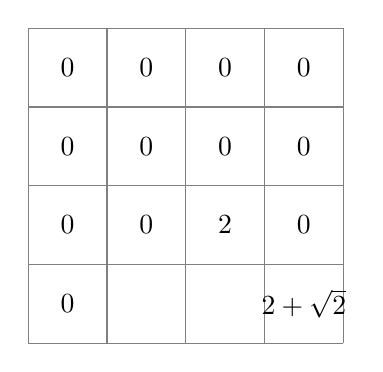
\begin{tikzpicture}
      \draw[step=1cm,color=gray] (-2,-2) grid (2,2);

      \node at (-1.5,+1.5) {$0$};
      \node at (-0.5,+1.5) {$0$};
      \node at (+0.5,+1.5) {$0$};
      \node at (+1.5,+1.5) {$0$};

      \node at (-1.5,+0.5) {$0$};
      \node at (-0.5,+0.5) {$0$};
      \node at (+0.5,+0.5) {$0$};
      \node at (+1.5,+0.5) {$0$};

      \node at (-1.5,-0.5) {$0$};
      \node at (-0.5,-0.5) {$0$};
      \node at (+0.5,-0.5) {$2$};
      \node at (+1.5,-0.5) {$0$};
      % ...
      \node at (-1.5,-1.5) {$0$};
      \node at (-0.5,-1.5) {};
      \node at (+0.5,-1.5) {};
      \node at (+1.5,-1.5) {$2 + \sqrt{2}$};
    \end{tikzpicture}
  }

  \subfloat[Initial state]{
    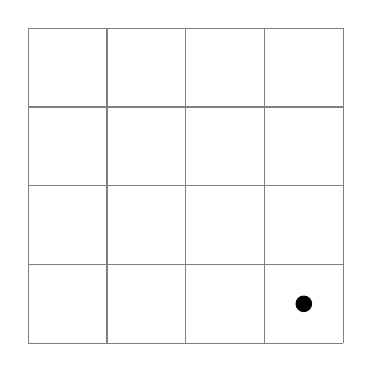
\begin{tikzpicture}
      \draw[step=1cm,color=gray] (-2,-2) grid (2,2);
      \fill[black] (1.5,-1.5) circle (3pt);   % value 14

    \end{tikzpicture}
  }
  \subfloat[Bifurcating condition]{
    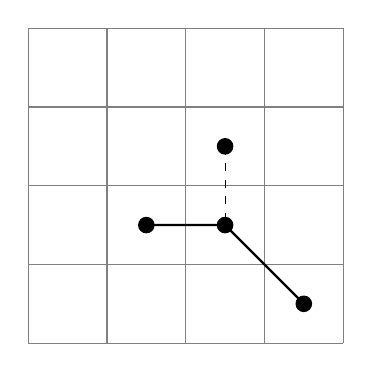
\begin{tikzpicture}
      \draw[step=1cm,color=gray] (-2,-2) grid (2,2);
      % Mark cells with flow accumulation ≥ 4 as red dots
      \fill[black] (0.5,0.5) circle (3pt);    % value 4
      \fill[black] (-0.5,-0.5) circle (3pt);  % value 5
      \fill[black] (0.5,-0.5) circle (3pt);   % value 12
      \fill[black] (1.5,-1.5) circle (3pt);   % value 14

      % Draw the main centerline along the highest accumulated path
      \draw[black,thick] (-0.5,-0.5) -- (0.5,-0.5) -- (1.5,-1.5);
      \draw[black,dashed] (0.5,0.5) -- (0.5,-0.5);
    \end{tikzpicture}
  }
  \subfloat[Bifurcated state]{
    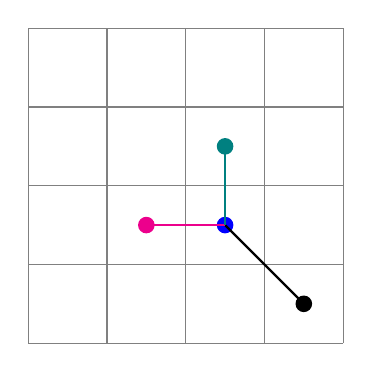
\begin{tikzpicture}
      \draw[step=1cm,color=gray] (-2,-2) grid (2,2);
      % Mark cells with flow accumulation ≥ 4 as red dots
      \fill[teal] (0.5,0.5) circle (3pt);    % value 4
      \fill[magenta] (-0.5,-0.5) circle (3pt);  % value 5
      \fill[blue] (0.5,-0.5) circle (3pt);   % value 12
      \fill[black] (1.5,-1.5) circle (3pt);   % value 14

      % Draw the main centerline along the highest accumulated path
      \draw[black,thick] (0.5,-0.5) -- (1.5,-1.5);
      \draw[magenta,thick] (-0.5,-0.5) -- (0.5,-0.5);
      \draw[teal,thick] (0.5,0.5) -- (0.5,-0.5);
    \end{tikzpicture}
  }

\end{figure}
\end{document}
